\section{Descrizione dei dati}
Il \textbf{modello dei dati} è l'insieme delle tecniche e 
dei costrutti usati per organizzare i dati e descriverne la loro natura. \\
Per esempio il \textbf{modello relazionale} ci permette di costruire 
\textbf{record} omogenei; vediamo un esempio.

\begin{center}
  \textbf{Orario} \\ \vspace{4px}
  \begin{tabular}{|l|c|r|}
    \hline
    Insegnamento & Docente & Aula \\ \hline
    Analisi I & Luigi Neri & N1 \\
    Chimica & Piero Rossi & N2 \\ 
    Basi di Dati & Angela Valenti & N3 \\
    Fisica II & Vittorio Strano & N4 \\ \hline
  \end{tabular}
\end{center}

La \emph{relazione} di cui parla il modello non è altro che l'intera 
tabella Orario, ed è composta da righe omogenee, ovvero righe che hanno
la stessa struttura: un \textbf{insegnamento}, un \textbf{docente} 
e un \textbf{aula}. \\
Sempre considerando la tabella possiamo adesso dare la definizione di 
\textbf{tupla} o (\textbf{record}) e \textbf{attributo}: la prima non 
è altro che una riga della tabella e la seconda è invece una colonna.
\\
\\
In ogni base di dati possiamo individuare uno \textbf{schema}, ovvero 
una \textit{descrizione} invariante nel tempo che descrive la struttura della
relazione; nella relazione \textit{Orario} vista prima lo schema è l'insieme
di \underline{tutti} gli attributi (ovvero le colonne della relazione). \\
Troveremo inoltre l'\textbf{istanza}, che è invece variabile nel tempo, ovvero
i valori della tabella stessa; la colonna \textit{Insegnamento} è per esempio una istanza.
\\
\\
Abbiamo già parlato del \textit{modello relazionale}, ma questo tipo fa in
realtà parte di una macro-categoria di modelli chiamati \textbf{modelli logici},
che descrivrono i dati, e le relazioni tra loro, usando strutture "comprensibili" 
ad un software (per esempio tramite \textbf{XML}). \\
Un'altra catergoria è quella dei \textbf{modelli concettuali} che invece mirano 
soltanto a rappresentare i dati a livello grafico, usando per esempio il famoso 
\textbf{schema E-R}, \textit{Entità-Relazione}. \\
Di seguito vedremo una archittetura molto comune per i DBMS, chiamata 
archittetura \textbf{ANSI/SPARC}:

\begin{center}
  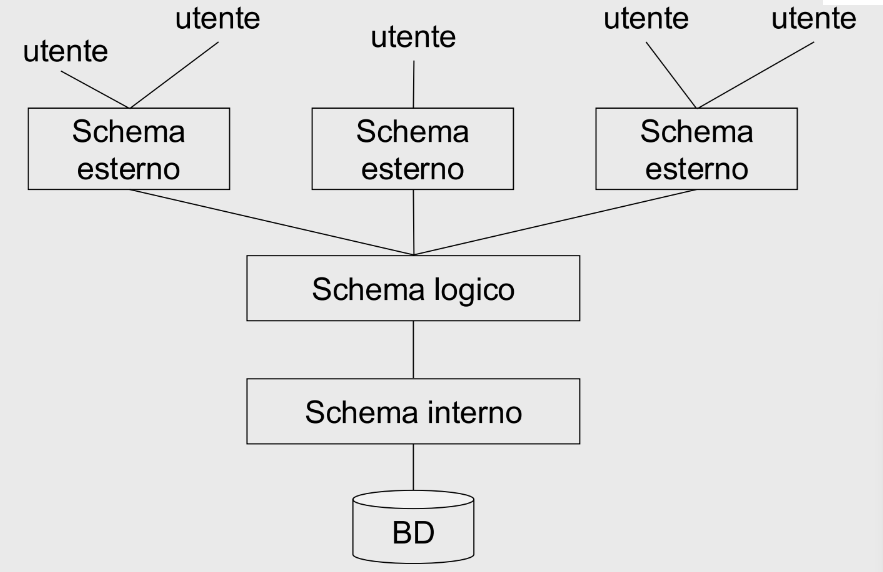
\includegraphics[width=0.8\textwidth]{descrizione-dei-dati/ANSI.png}
\end{center}

Ogni schema dell'archittetura ha una sua funzione e soprattutto lavora 
soltanto su una parte del database. \\
Lo \textbf{schema esterno} è quello a cui si interfaccierà l'utente, di 
conseguenza sarà molto "semplificato". Se per esempio prendiamo il sito di
una università l'utente medio sarà uno studente, lo schema esterno lavorerà
quindi (e farà vedere) soltanto sui voti di quello studente; il database
dell'università ha ovviamente altri dati (nomi dei professori, eventi, 
gli esami degli scorsi anni), ma farà solo vedere allo studente ciò che
a lui davvero serve. \\
Al cuore della struttura troviamo invece lo \textbf{schema logico}
che descrive in modo concettuale quali sono i dati e le relazioni tra 
quest'ultimi (per esempio tramite il \textit{modello ER}, come detto prima) \\
L'ultimo è lo \textbf{schema interno} che descrive come sono 
\textit{fisicamente} memorizzati questi dati e su quali dispostivi
(\textit{HDD}, \textit{SDD} etc)
\\
Il punto forte di questa struttura è l'\textbf{indipendenza dei dati}, 
infatti potremmo cambiare il modo in cui "descriviamo i dati" (schema logico),
senza cambiare poi gli altri schemi o addirittura il database stesso.